\bichapter{改性纳米铁在多孔介质的迁移性能研究}{Migration properties of modified iron nanoparticles in porous media}

\bisection{材料制备和研究方法}{Materials and methods}

使用粒度为0.55-1 mm的高纯石英砂作为多孔介质。在使用之前,用6 M HCl溶液处理砂子24 h以去除杂质,然后用去离子水反复冲洗,直到冲洗水中$\mathrm{pH}>5.5$。迁移实验均以3 mM NaCl为背景溶液,在内径为3 cm、长度为30 cm的石英砂填充玻璃柱中进行,实验装置如\cref{column}所示。立柱两端装分别填充直径为0.3 cm的玻璃珠以保证布水均匀。进出口处连接测压管用于检测进出口水头。连接蠕动泵将液体泵入柱中,流动方向为从柱底流向柱顶。

在每次迁移实验之前,用3mM NaCl背景溶液冲洗填料柱至少10个孔隙体积(PVs)。之后用约3 PVs (120 mL)的示踪剂(25 mg/L $\mathrm{KNO_3}$)测定色谱柱的分散性和孔隙率。每5分钟测定出水溶液中$\mathrm{NO^{3-}}$的浓度。将示踪剂浓度归一化,拟合穿透曲线曲线,得到砂柱的平均扩散系数。

为了验证再释放效果,SA-NZVI和SA-S-NZVI分别以5、10、15 mL/min流速的注射条件下,将5 PVs的悬浮液注入柱中。随后将70 PVs背景溶液以相同流速泵入柱中,以洗脱柱中颗粒。将上述操作重复三次,以一定时间间隔读取测压管水头,并收集流出物,并使用盐酸溶解以分析铁的浓度。为确保颗粒稳定性,注射过程中使用电动搅拌机以520 r/min速率持续搅拌。定时测量颗粒的平均水动力粒径($a_\mathrm{h}$)。每次结束后,仔细将砂柱按照长度方向分为10段,使用6 M HCl消解。使用紫外分光光度法测试溶液总铁浓度以测量砂柱中沉积的NZVI/S-NZVI的空间分布,并对比多次注入/冲洗后NZVI/S-NZVI在砂柱残留的质量差异和过程中测压管水头变化。

\begin{figure}[h]
    \centering
    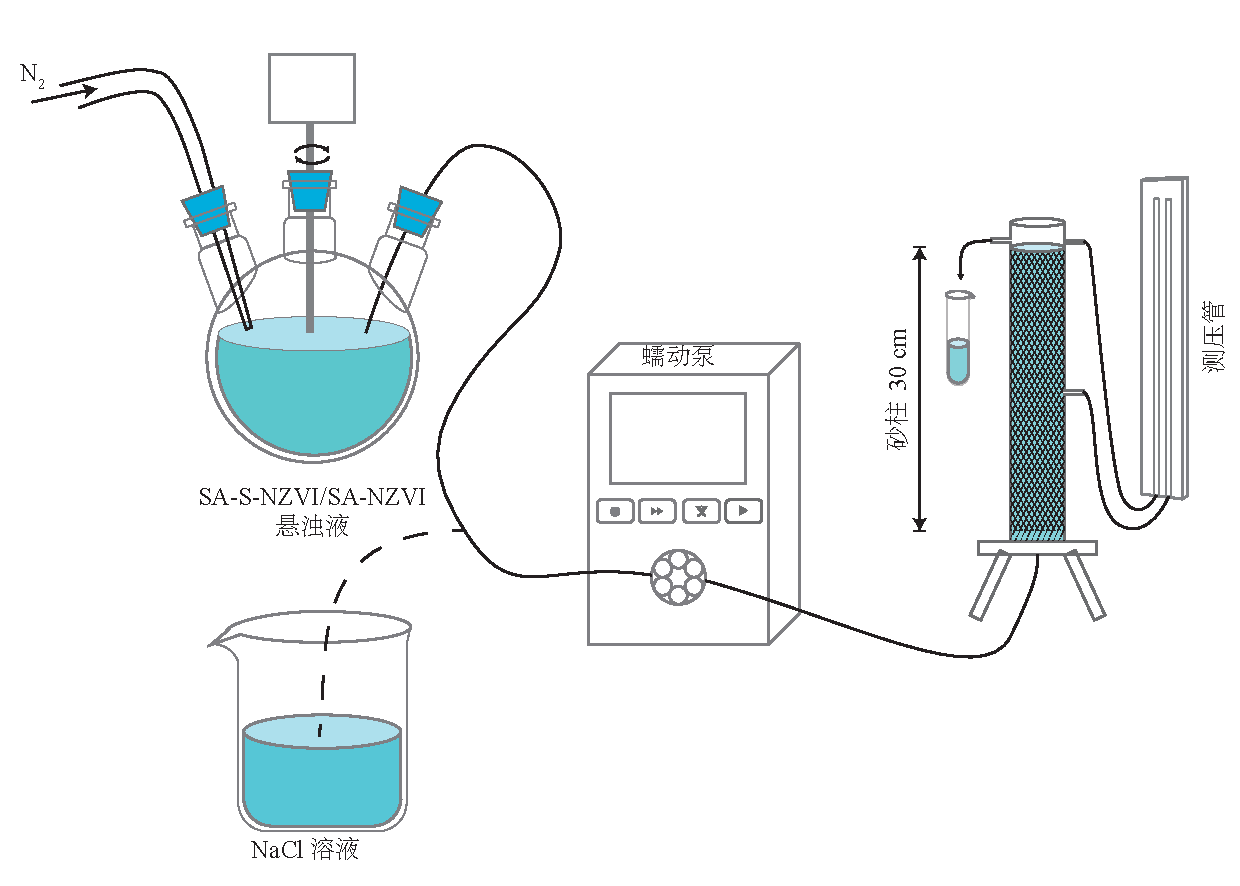
\includegraphics[width=12cm]{figs/column.pdf}
    \bicaption{柱实验装置示意图}{Schematic diagramm of the experimental device}
    \label{column}
\end{figure}

